\documentclass[preview]{standalone}
\usepackage{amsmath}
\usepackage{amssymb}
\usepackage{stellar}
\usepackage{definitions}
\usepackage{bettelini}
\usepackage{tikz}
\usepackage{pgfplots}
\pgfplotsset{compat=1.18}
\begin{document}
\id{diffeq-function-space-exercises}
\genpage
\section{Exercises}

\begin{snippetexercise}{diffeq-norm-convergence-exercise}{Convergence in different norms}
    For \(n\geq1\), let
    \[
        f_n(x)=e^{x^3/n}+\tanh(nx)-\frac{\cos(nx)}{n^2}.
    \]
    Determine convergence in \(C^0([a,b])\), \(C^1([a,b])\), \(C^2([a,b])\),
    for \(a<b\), and convergence of \(f_n\) and \(f_n'\) in \(B((-\infty,-1))\).
\end{snippetexercise}

\begin{snippetsolution}{diffeq-norm-convergence-solution}{Pointwise and uniform convergence}
    Pointwise \(e^{x^3/n}\to1\), \(\cos(nx)/n^2\to0\), while
    \(\tanh(nx)\to-1,0,1\) according as \(x<0,x=0,x>0\). Hence
    \[
        f(x)=\begin{cases}0,&x<0,\\1,&x=0,\\2,&x>0.\end{cases}
    \]
\begin{center}
\begin{tikzpicture}[x=1.1cm,y=0.8cm]
	\draw[->] (-3.2,0) -- (3.2,0) node[right] {\(x\)};
	\draw[->] (0,-0.5) -- (0,2.7) node[above] {\(f(x)\)};
	\draw[thick] (-3,0) -- (-0.12,0);
	\draw[thick] (0.12,2) -- (3,2);
	\draw[fill=white,thick] (0,0) circle (2pt);
	\filldraw (0,1) circle (2pt) node[right] {\(1\)};
	\draw[fill=white,thick] (0,2) circle (2pt);
	\node[left] at (0,2) {\(2\)};
\end{tikzpicture}
\end{center}
    If \(a<b<0\), write
    \(f_n=(e^{x^3/n}-1)+(1+\tanh(nx))-\cos(nx)/n^2\), and use
    \[
        |e^{x^3/n}-1|\leq1-e^{a^3/n},\quad
        |1+\tanh(nx)|\leq1+\tanh(nb),\quad
        |\cos(nx)/n^2|\leq n^{-2}.
    \]
    All three bounds tend to zero. For \(0<a<b\), write \(f_n-2\) instead,
    and use \(e^{b^3/n}-1\), \(1-\tanh(na)\), \(n^{-2}\).
    Thus convergence in \(C^0([a,b])\) holds exactly when \(b<0\) or \(a>0\).
    If \(0\in[a,b]\), even as an endpoint, the pointwise limit is not continuous,
    excluding uniform convergence.
\end{snippetsolution}

\begin{snippetsolution}{diffeq-norm-derivative-solution}{First and second derivatives}
    For \(f_n=e^{x^3/n}+\tanh(nx)-\cos(nx)/n^2\),
    \[
        f_n'=\frac{3x^2}{n}e^{x^3/n}
               +n(1-\tanh^2(nx))+\frac{\sin(nx)}n.
    \]
    On \(a<b<0\), the three terms have bounds
    \(3a^2/n\), \(n(1-\tanh^2(nb))\), \(1/n\).
    On \(0<a<b\), use \(3b^2e^{b^3/n}/n\),
    \(n(1-\tanh^2(na))\), \(1/n\).
    Exponential decay of \(1-\tanh^2(nc)\), \(c>0\), makes these bounds vanish.
    Consequently convergence in \(C^1\) holds exactly on intervals avoiding zero,
    with the same constant limits \(0\) or \(2\).

    Differentiating again,
    \[
        f_n''=\frac3n e^{x^3/n}\left(\frac{3x^4}n+2x\right)
        -2n^2\tanh(nx)(1-\tanh^2(nx))+\cos(nx).
    \]
    Away from zero the first two terms tend uniformly to zero.
    The last cannot converge uniformly on any nondegenerate interval:
    for large \(n\) choose \(x_n,y_n\) in it with
    \(|x_n-y_n|=\pi/n\), \(\cos(nx_n)=1\), \(\cos(ny_n)=-1\).
    Uniform convergence to a continuous limit would force their value difference
    to tend to zero, a contradiction.
    Intervals containing zero already fail in \(C^0\).
    Hence there is no \(C^2([a,b])\) convergence for any \(a<b\).
\end{snippetsolution}

\begin{snippetsolution}{diffeq-norm-halfline-solution}{The unbounded half-line}
    On \((-\infty,-1)\), the pointwise limit of
    \(f_n=e^{x^3/n}+\tanh(nx)-\cos(nx)/n^2\) is zero, but
    \[
        f_n(-n)=e^{-n^2}-\tanh(n^2)-\frac{\cos(n^2)}{n^2}\longrightarrow-1.
    \]
    Thus convergence in \(B((-\infty,-1))\) fails.
    For the derivatives, the sine term is bounded by \(1/n\), and
    \[
        0\leq n(1-\tanh^2(nx))\leq n(1-\tanh^2 n)\longrightarrow0.
    \]
    For the exponential term put \(t=x/n^{1/3}\). Then
    \[
        \frac{3x^2}n e^{x^3/n}=3n^{-1/3}g(t),\qquad
        g(t)=t^2e^{t^3},\quad t<0.
    \]
    This positive \function tends to zero at both ends of \((-\infty,0)\).
    Since \(g'(t)=te^{t^3}(2+3t^3)\),
    \[
        \max_{t<0}g(t)=\left(\frac23\right)^{2/3}e^{-2/3}=:M.
    \]
    Therefore the supremum of the exponential term is at most \(3Mn^{-1/3}\).
    All terms of \(f_n'\) tend uniformly to zero on the half-line.
    The original schematic drawing indicates the moving maximum.
\begin{center}
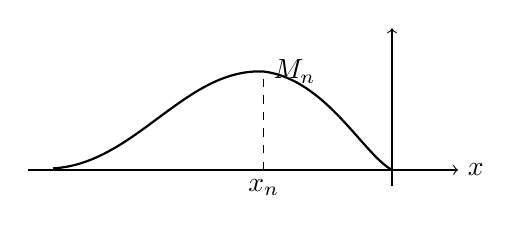
\begin{tikzpicture}[x=1.05cm,y=1cm]
	\draw[->] (-4.4,0) -- (0.8,0) node[right] {\(x\)};
	\draw[->] (0,-0.2) -- (0,1.8);
	\draw[thick] (-4.1,0.02) .. controls (-3.1,0.08) and (-2.5,1.3) .. (-1.55,1.25)
		.. controls (-0.8,1.15) and (-0.35,0.2) .. (0,0);
	\draw[dashed] (-1.55,0) -- (-1.55,1.25);
	\node[below] at (-1.55,0) {\(x_n\)};
	\node[right] at (-1.55,1.25) {\(M_n\)};
\end{tikzpicture}
\end{center}
\end{snippetsolution}

\end{document}
